\beginsong{Der Piet am Galgen hängt}[wuw={Erik Martin, 1981}, bo={364}, pfii={69}, pfiii={25}, gruen={196}, kssiv={46}, siru={252}, index={Piet am Galgen, Was kann ich denn dafür}]

\beginverse 
\endverse
\centering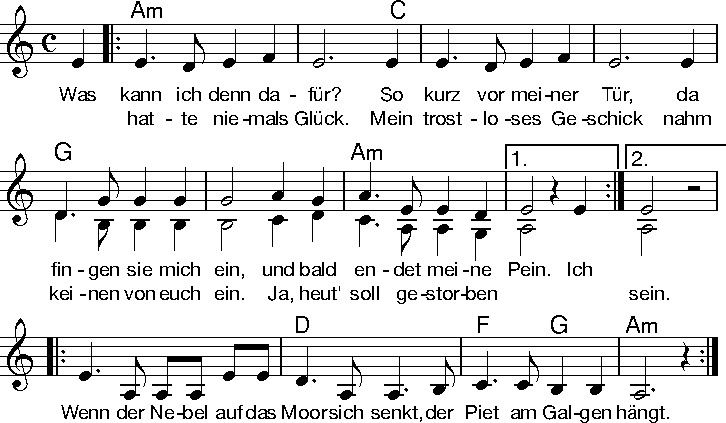
\includegraphics[width=1\textwidth]{Noten/Lied019.pdf}	

\beginverse
Sie \[Am]nahmen mir die Schuh' und \[C]auch den Rock dazu.
Sie \[G]banden mir die Händ' und mein \[Am]Haus, es hat gebrennt. 
Ich \[Am]sah den Galgen steh'n. Sie \[C]zwangen mich zu geh'n. 
Sie \[G]wollten meinen Tod, keiner \[Am]half mir in der Not.
\endverse

\beginchorus
\lrep \[Am]Wenn der Nebel auf das \[D]Moor sich senkt, der \[F]Piet am \[G]Galgen \[Am]hängt.\rrep
\endchorus

\beginverse
Was ^kratzt da am Genick? Ich ^spür' den rauhen Strick.
Ein ^Mönch der betet dort und spricht ^für mich fromme Wort,
die Wort, die ich nicht kenn', wer ^lehrte sie mich denn? 
Fünf ^Raben fliegen her, doch ich ^sehe sie nicht mehr.
\endverse

%\renewcommand{\everychorus}{\textnote{\bf Refrain (wdh.) }}
\beginchorus
\lrep \[Am]Wenn der Nebel auf das \[D]Moor sich senkt, der \[F]Piet am \[G]Galgen \[Am]hängt.\rrep
\endchorus

\endsong

\beginscripture{}
Der Verfasser lässt im Unklaren, auf wen sich die Person des Piet tatsächlich bezieht. Es sind jedoch Parallelen zum Schinderhannes erkennbar.
\endscripture

\begin{intersong}
\ifthenelse{\boolean{pics}}{
    \vspace{25pt}
    \centering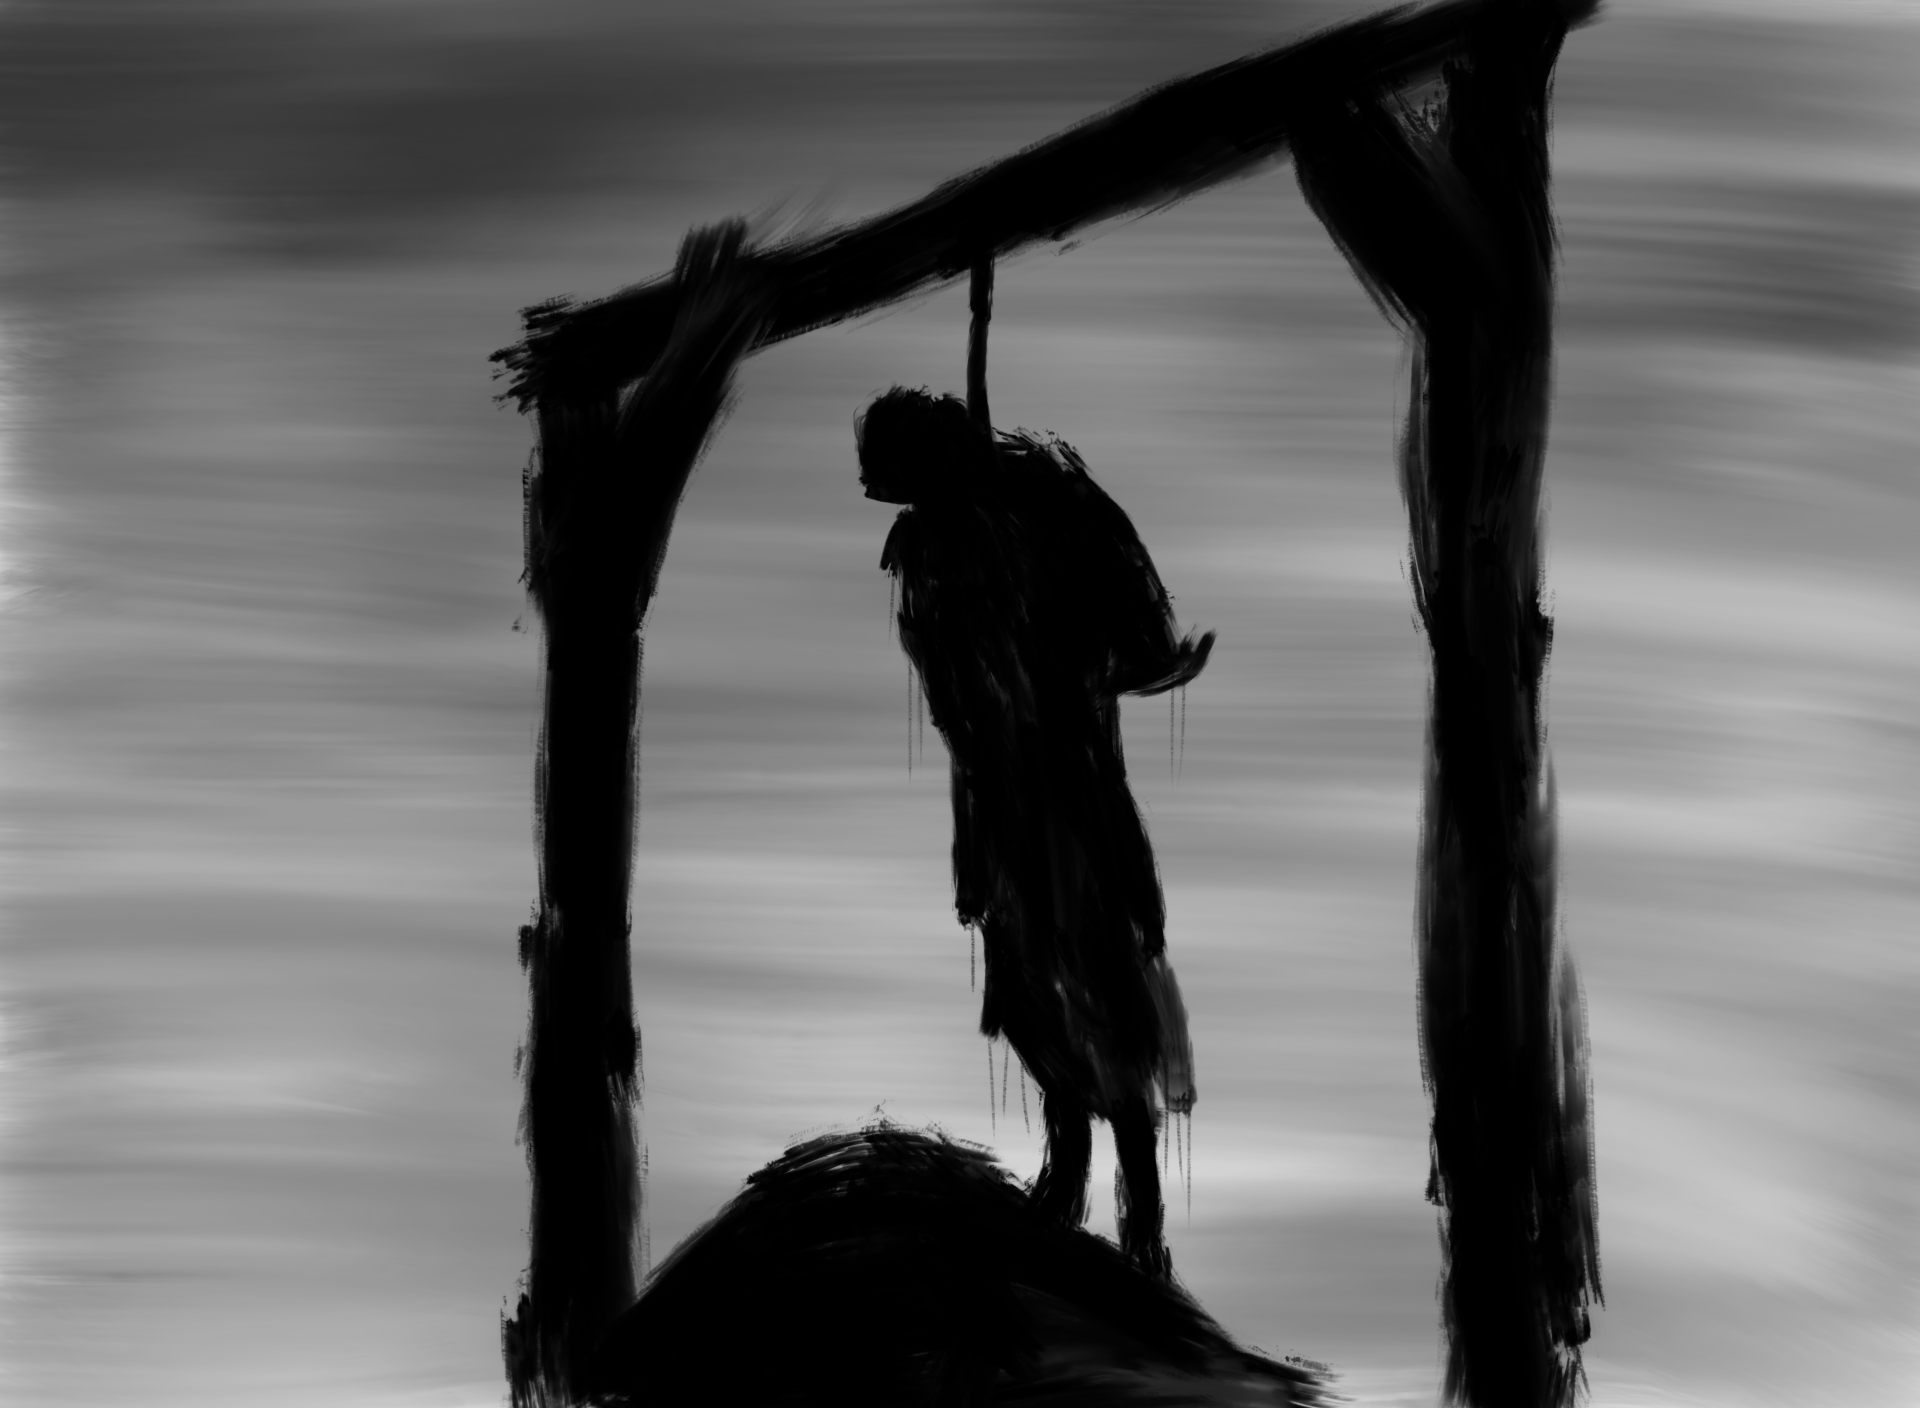
\includegraphics[width=1\textwidth]{Bilder/piet_heiko.png}	
}{}
\end{intersong}